\section{Como representar algoritmos?}

\begin{frame}{Formas de representação}
  Existem no mínimo duas formas bem difundidas de como representar algoritmos: \textbf{Linguagem natural}, \textbf{Fluxograma} e \textbf{Pseudocódigo}.
  \begin{itemize}
    \item \textbf{Linguagem natural}: o Algoritmo é escrito em frases comuns, como uma explicação passo a passo. Por exemplo, \textit{\color{blue}Para encontrar o maior número em uma lista, percorra cada elemento e compare com o maior já encontrado. Se for maior, atualize. No final, o maior número será o resultado.}.
  \end{itemize}
\end{frame}

\begin{frame}{Formas de representação}
  Existem no mínimo duas formas bem difundidas de como representar algoritmos: \textbf{Linguagem natural}, \textbf{Fluxograma} e \textbf{Pseudocódigo}.
  \begin{itemize}
    \item \textbf{Fluxograma}: os algoritmos são representados de forma visual usando diagramas que representam o fluxo de execução do algoritmo.
  \end{itemize}
  \begin{figure}
    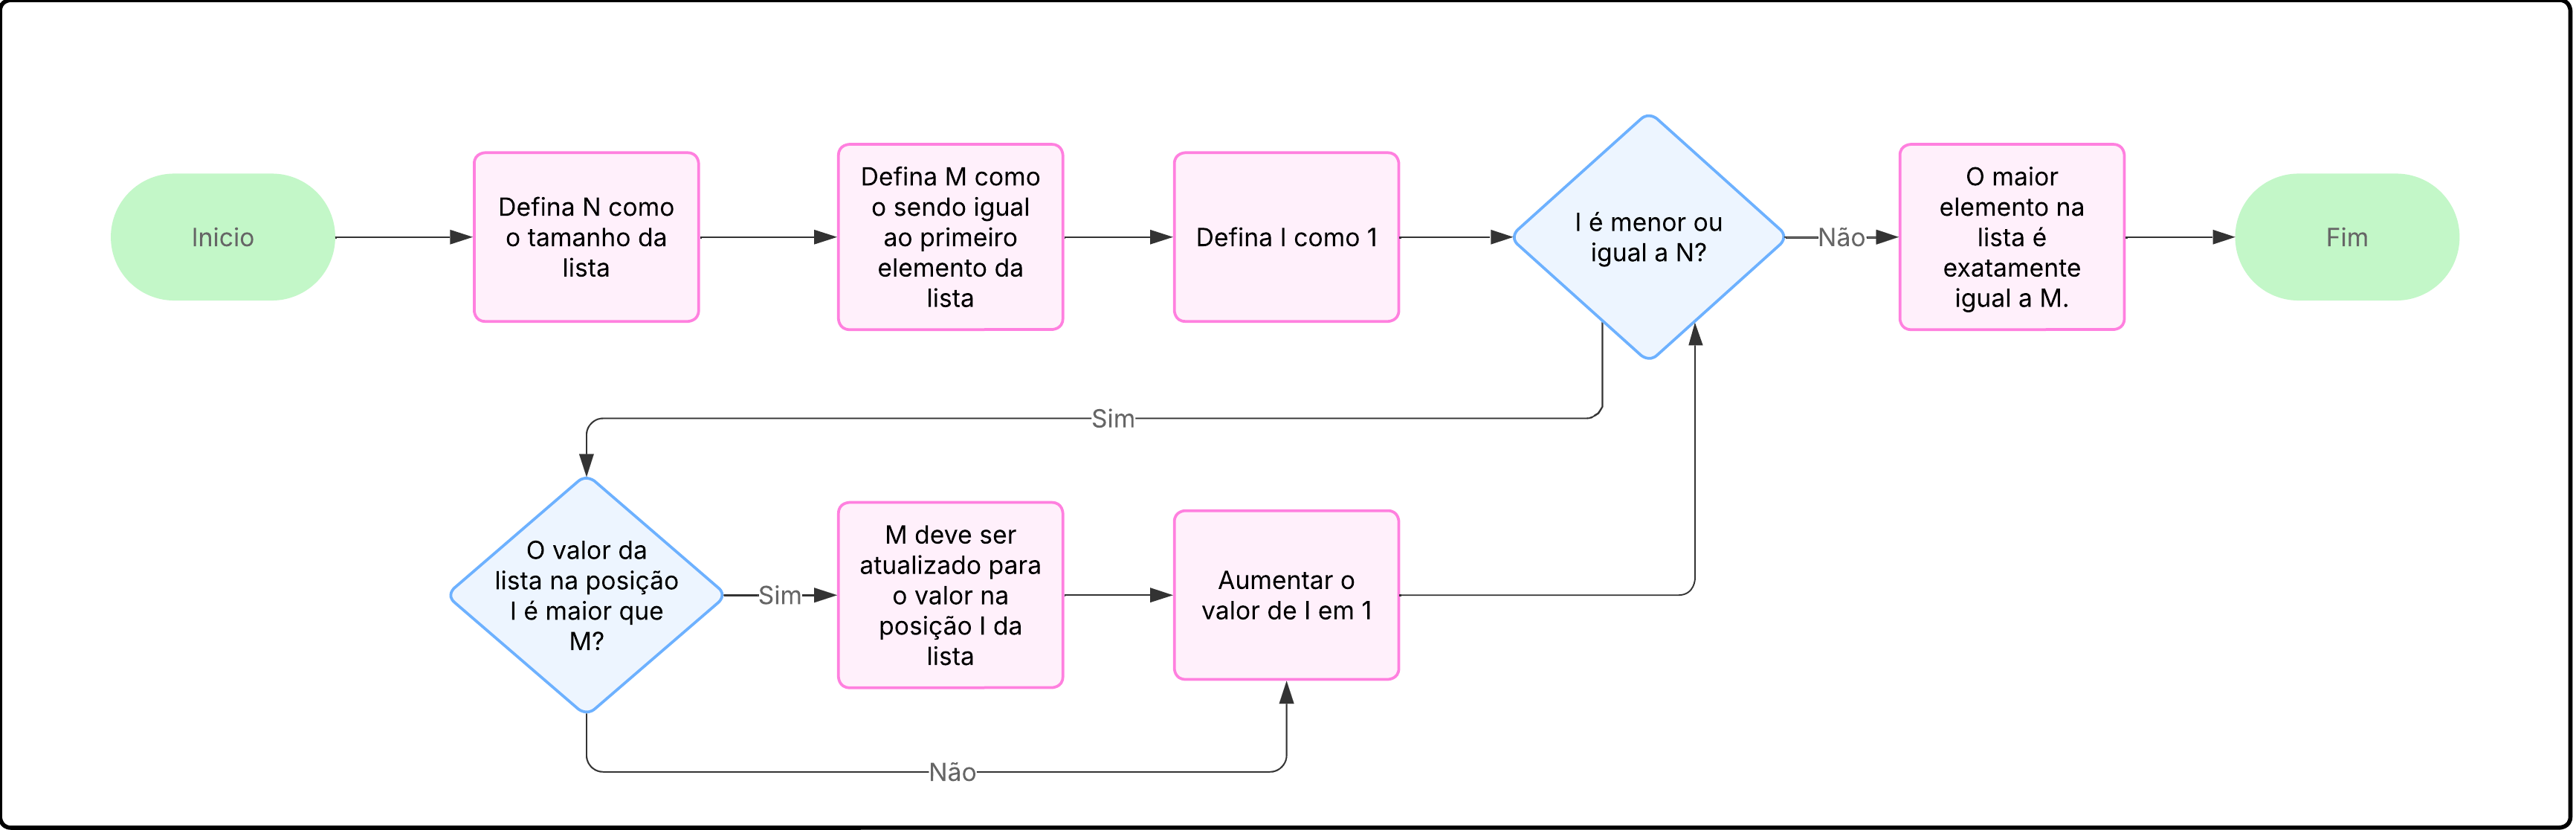
\includegraphics[width=0.85\textwidth]{figuras/Fluxograma}
  \end{figure}
\end{frame}

\begin{frame}{Sobre os fluxogramas}
  Os símbolos padronizados usados no fluxograma podem ser compreendidos da seguinte forma:
  \begin{enumerate}
    \item Elipse: indica o ponto inicial e o ponto final do fluxograma.
    \item Retângulo: representa uma operação ou ação, como calcular, armazenar um valor ou executar uma tarefa.
    \item Paralelogramo: indica operações de entrada (como receber dados do usuário) e saída (mostrar um resultado).
    \item Losango: representa um ponto onde o fluxo pode seguir diferentes direções, dependendo de uma condição lógica.
  \end{enumerate}
\end{frame}

\begin{frame}{Formas de representação}
  Existem no mínimo duas formas bem difundidas de como representar algoritmos: \textbf{Linguagem natural}, \textbf{Fluxograma} e \textbf{Pseudocódigo}.
  \begin{itemize}
    \item \textbf{Pseudocódigo}:  é uma forma estruturada de representar algoritmos utilizando uma mistura de linguagem natural e elementos de linguagens de programação.
  \end{itemize}
\end{frame}

\begin{frame}{Exemplo de Pseudocódigo}
  \begin{algorithm}[H]
    \SetAlgoLined
    \Entrada{A lista $L$ de tamanho $N$} 
    \Saida{O maior valor em $L$}
    \Inicio{
      $i = 1$\\
      $M = L[0]$\\
      \Enqto{$i < N$}{
        \Se{$L[i] > M$}{
          $M = L[i]$\\
        }
      }
    }
    \Retorna{$M$}
    \label{alg1}
    \caption{Algoritmo para encontrar o maior valor na lista.}
  \end{algorithm}
\end{frame}

